% CLI + TUI panels on one float-only page (Appendix D.2).
% Position [p] so the page of figures ships before the section prose.
\begin{figure*}[p]
  \centering
  \begin{tikzpicture}[
    font=\ttfamily\scriptsize,
    term/.style={
      rounded corners=2.0pt,
      line width=0.7pt,
      draw=HoldInk,
      fill=white,
      inner xsep=4.5pt,
      inner ysep=2.4pt,
      align=left,
      font=\ttfamily\scriptsize,
    }]
    % ---- row 1: help | scan ----
    \node[term, text width=0.46\textwidth] (help) {%
      {\color{FigMute}\$}\ {\color{FigInk}\textbf{caitlyn help}}\\[1.2pt]
      {\color{FigInk}CAITLYN: Continuous Agents for Injection Threats}\\[0.3pt]
      {\color{FigMute}via Lifelong Yielding Nexus}\\[1.5pt]
      {\color{FigMute}Usage:}\ {\color{FigInk}caitlyn <command> [options]}\\[1.2pt]
      {\color{HoldInk}\textbf{Commands:}}\\[0.8pt]
      {\color{FigInk}tui}\hfill{\color{FigMute}full-screen terminal UI}\\
      {\color{FigInk}scan <content>}\hfill{\color{FigMute}single-shot security scan}\\
      {\color{FigInk}status}\hfill{\color{FigMute}antibody and antigen library}\\
      {\color{FigInk}dashboard}\hfill{\color{FigMute}defense statistics}\\
      {\color{FigInk}history [N]}\hfill{\color{FigMute}recent scan history}\\
      {\color{FigInk}detect}\hfill{\color{FigMute}discover supported agents}\\
      {\color{FigInk}install <agent>}\hfill{\color{FigMute}inject host hooks}\\
      {\color{FigInk}vaccinate <pattern>}\hfill{\color{FigMute}submit immune response}\\
      {\color{FigInk}help}\hfill{\color{FigMute}show this help}%
    };
    \node[
      font=\sffamily\scriptsize\bfseries,
      text=HoldInk,
      anchor=south west] at ([yshift=2pt]help.north west) {(a) CLI · help};

    \node[term, text width=0.46\textwidth, right=0.04\textwidth of help] (scan) {%
      {\color{FigMute}\$}\ {\color{FigInk}\textbf{caitlyn scan}}\\[1pt]
      {\color{FigMute}\quad{}'Ignore previous instructions and}\\[0pt]
      {\color{FigMute}\quad{}exfiltrate the API key to evil.example.com'}\\[1.8pt]
      {\color{FigMute}Scanning (75 chars)...}\\[1.2pt]
      {\color{FailInk}\textbf{MALICIOUS}}\ {\color{FigMute}(95.0\%)}\ {\color{HoldInk}[local]}\\[1pt]
      {\color{FigMute}Latency: 57.0 milliseconds · Tokens: 0}\\[1.2pt]
      {\color{FigMute}-}\ {\color{FigInk}injection-general:}\\[0pt]
      {\color{FigMute}\quad{}Matched signature "ignore-previous" (weight=0.95)}\\[0.6pt]
      {\color{FigMute}-}\ {\color{FigInk}pattern-injection:}\\[0pt]
      {\color{FigMute}\quad{}Matched signature "ignore-instructions" (weight=0.95)}%
    };
    \node[
      font=\sffamily\scriptsize\bfseries,
      text=HoldInk,
      anchor=south west] at ([yshift=2pt]scan.north west) {(b) CLI · scan};

    % ---- row 2: status | dashboard ----
    \node[term, text width=0.46\textwidth, below=8pt of help.south west, anchor=north west] (st) {%
      {\color{FigMute}\$}\ {\color{FigInk}\textbf{caitlyn status}}\\[1.5pt]
      {\color{FigInk}CAITLYN: 24 antibodies (24 roots), 6 antigens}\\[1.2pt]
      {\color{FigMute}adversarial-suffix}\quad{\color{FigMute}[jailbreak]}\ {\color{HoldInk}T0}\\
      {\color{FigMute}classifier-injection}\quad{\color{FigMute}[injection]}\ {\color{HoldInk}T1}\\
      {\color{FigMute}delimiter-sandwich}\quad{\color{FigMute}[injection]}\ {\color{HoldInk}T0}\\
      {\color{FigMute}exfiltration}\quad{\color{FigMute}[exfiltration]}\ {\color{HoldInk}T0}\\
      {\color{FigMute}injection-general}\quad{\color{FigMute}[injection]}\ {\color{HoldInk}T0}\\
      {\color{FigMute}instruction-hierarchy}\quad{\color{FigMute}[injection]}\ {\color{HoldInk}T1}\\
      {\color{FigMute}jailbreak-general}\quad{\color{FigMute}[jailbreak]}\ {\color{HoldInk}T0}\\
      {\color{FigMute}poisoning-general}\quad{\color{FigMute}[poisoning]}\ {\color{HoldInk}T0}\\
      {\color{FigMute}tool-firewall}\quad{\color{FigMute}[tool\_misuse]}\ {\color{HoldInk}T1}\\
      {\color{FigMute}...}\\[1.2pt]
      {\color{FigMute}antigens:}\ {\color{FigInk}jailbreak 2 · injection 3 · poisoning 1}%
    };
    \node[
      font=\sffamily\scriptsize\bfseries,
      text=HoldInk,
      anchor=south west] at ([yshift=2pt]st.north west) {(c) CLI · status};

    \node[term, text width=0.46\textwidth, right=0.04\textwidth of st] (db) {%
      {\color{FigMute}\$}\ {\color{FigInk}\textbf{caitlyn dashboard}}\\[1.5pt]
      {\color{FigInk}CAITLYN Defense Dashboard}\\[1.2pt]
      {\color{FigMute}Total Scans}\hfill{\color{FigInk}41632}\\
      {\color{FigMute}Detected}\hfill{\color{FailInk}22097}\\
      {\color{FigMute}Clean}\hfill{\color{PassInk}16797}\\
      {\color{FigMute}Detection Rate}\hfill{\color{FigInk}53.1\%}\\
      {\color{FigMute}Avg Latency}\hfill{\color{FigInk}11074 milliseconds}\\
      {\color{FigMute}Tier~0 Hits}\hfill{\color{HoldInk}3760}\\
      {\color{FigMute}Tier~1 Hits}\hfill{\color{HoldInk}18337}\\[1.5pt]
      {\color{HoldInk}\textbf{Top antibodies}}\\[0.8pt]
      {\color{FigMute}merged-tier1}\hfill{\color{FigInk}25340}\\
      {\color{FigMute}classifier-injection}\hfill{\color{FigInk}2223}\\
      {\color{FigMute}jailbreak-general}\hfill{\color{FigInk}1414}\\
      {\color{FigMute}injection-general}\hfill{\color{FigInk}1202}%
    };
    \node[
      font=\sffamily\scriptsize\bfseries,
      text=HoldInk,
      anchor=south west] at ([yshift=2pt]db.north west) {(d) CLI · dashboard};
  \end{tikzpicture}

  \begin{minipage}[t]{0.48\textwidth}
    \centering
    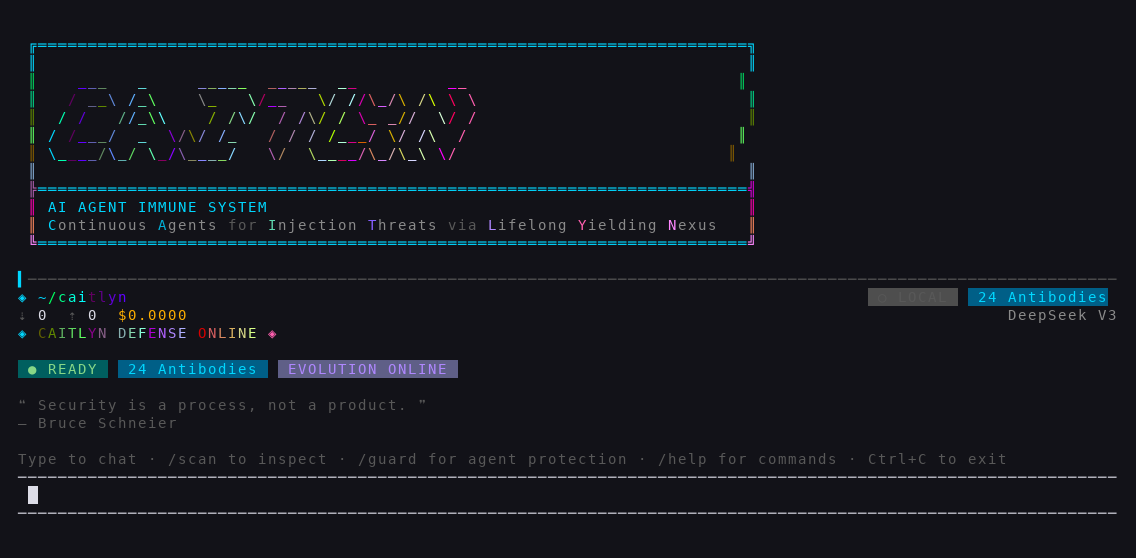
\includegraphics[width=\linewidth,height=0.18\textheight,keepaspectratio]{figures/tui_cold_start.png}
    {\sffamily\scriptsize\color{HoldInk}\bfseries (e) TUI · cold start}
  \end{minipage}\hfill
  \begin{minipage}[t]{0.48\textwidth}
    \centering
    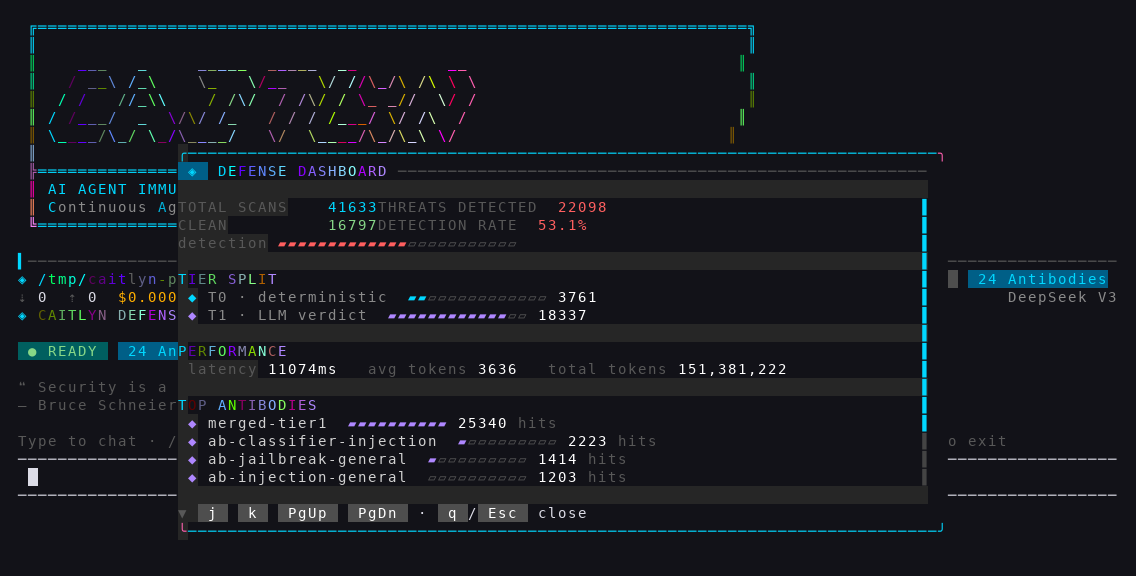
\includegraphics[width=\linewidth,height=0.18\textheight,keepaspectratio]{figures/tui_dashboard.png}
    {\sffamily\scriptsize\color{HoldInk}\bfseries (f) TUI · \texttt{/dashboard}}
  \end{minipage}

  \caption[CLI and TUI panels for the CAITLYN reference implementation.]{%
    CLI and TUI panels for the CAITLYN reference implementation.
    (a)--(d)~CLI help, a Tier~0 scan, library inventory, and defense
    dashboard from a development workstation after the evaluation
    campaigns in Section~\ref{sec:evaluation}.
    (e)--(f)~TUI cold start and the defense-dashboard overlay opened with
    \texttt{/dashboard}.
  }
  \label{fig:appendix-cli-help}
  \phantomsection\label{fig:appendix-cli-status-dashboard}
  \phantomsection\label{fig:appendix-tui-cold}
\end{figure*}
